\section{Stress}
The internal forces and moments generally vary from point to point. Obtaining this distribution is of primary importance in mechanics of materials. The total force in a cross-section, divided by the cross-sectional area, is the \textbf{stress}. We use stress to \textbf{normalize forces} with respect to the size of the geometry.

\subsection{Units}
The units of stress can be found in the table below.

\begin{figure*}[!h]
\centering
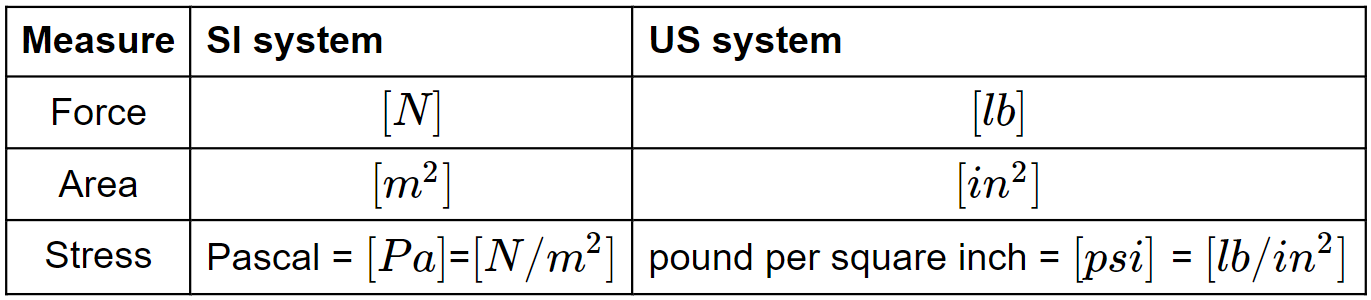
\includegraphics[angle=0, width=4in]{Stress-Figures/Units.png}
\vspace{-2mm}
\caption{\small Table screenshot from ref pages}
\vspace{-3mm}
\label{Table:Units}
\end{figure*}

\noindent It is also important to recall some of the most common prefixes used to denote quantity.

\begin{figure*}[!h]
\centering
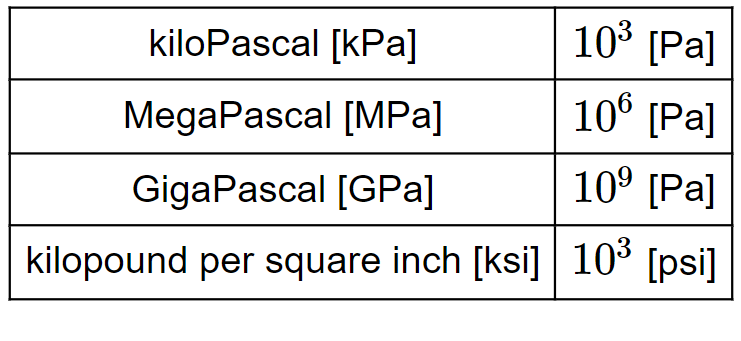
\includegraphics[angle=0, width=2in]{Stress-Figures/Prefixes.png}
\vspace{-2mm}
\caption{\small Table screenshot from ref pages}
\vspace{-3mm}
\label{Table:Prefixes}
\end{figure*}

\begin{itemize}
    \item \textbf{Tension:} $\sigma > 0$
    \item \textbf{Compression:} $\sigma < 0$
\end{itemize}
Typical sign convention for axial (normal) stress:

\subsection {Stress under general loading conditions}

We consider a homogeneous distribution of the internal force $\Delta F$ over an infinitesimal area $\Delta A$. The stress is defined by the infinitesimal force divided by the infinitesimal area.

\begin{itemize}
    \item \textbf{Normal Stress:} Defined by the intensity of the force acting NORMAL to $\Delta A$
    \item \textbf{Shear Stress:} Defined by the intensity of the force acting TANGENT to $\Delta A$
\end{itemize} 

\subsubsection{Average Normal Stress - Axial Loading}

\begin{figure*}[!h]
\centering
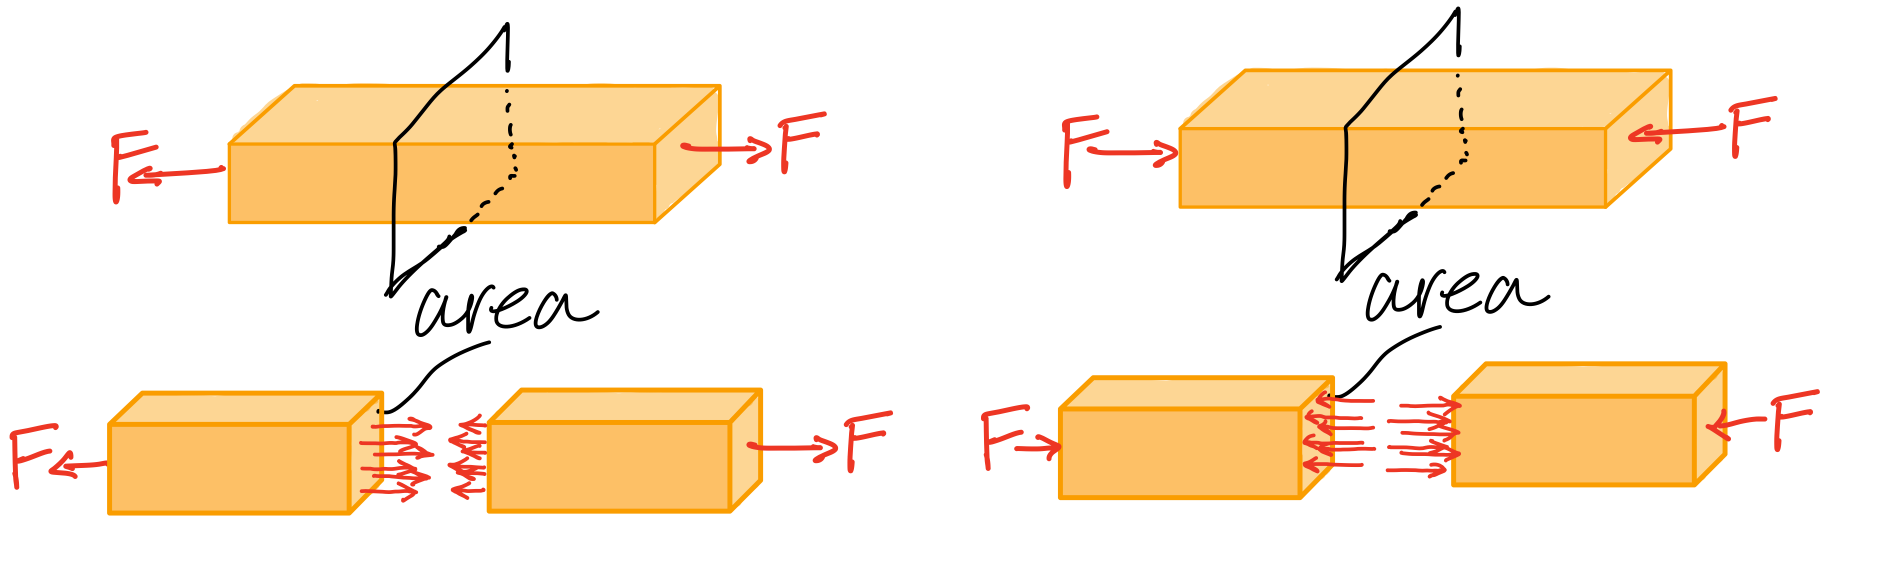
\includegraphics[angle=0, width=5in]{Stress-Figures/Normal Stress.png}
\vspace{-2mm}
\caption{\small Normal stress}
\vspace{-3mm}
\label{Fig:NormalStress}
\end{figure*}

\noindent Here we assume that the\textbf{ distribution of normal stresses} in an axially loaded member is \textbf{uniform}. Stress is calculated away from the points of application of the concentrated loads. Uniform distribution of stress is possible only if the line of action of the concentrated load $P$ passes through the centroid of the section considered

\[\sigma_{ave} = \frac{F}{A}\]

\noindent where $F$ is the internal resultant normal force and $A$ is the cross-sectional area of the bar where the normal stress $\sigma_{ave}$ is calculated.

\begin{figure*}[!h]
\centering
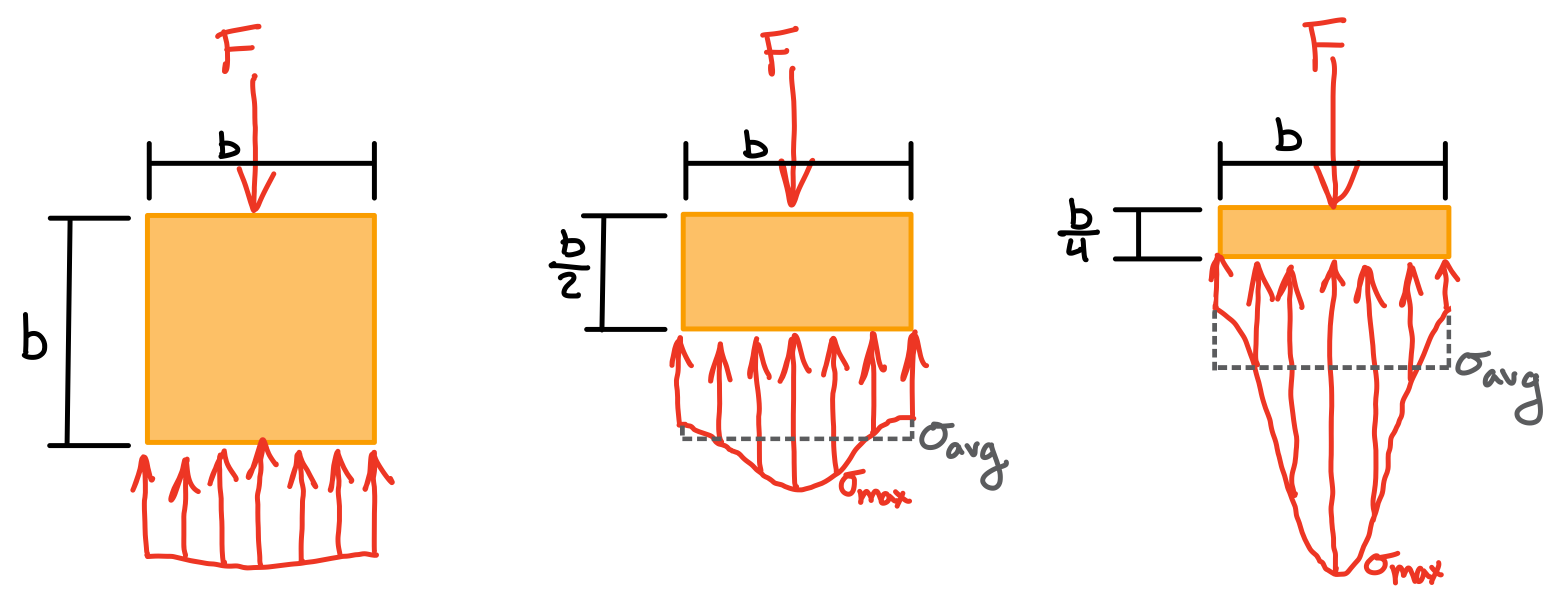
\includegraphics[angle=0, width=5in]{Stress-Figures/Stress Distribution.png}
\vspace{-2mm}
\caption{\small Non-uniform stress distribution}
\vspace{-3mm}
\label{Fig:StressDist}
\end{figure*}

\noindent Around the point where the load is applied, the stress distribution is non-uniform. Cross-sections farther away from the point load gradually have a more uniform distribution. When the distance is greater than the widest dimension of the cross-section ($l > b$), the stress distribution is uniform.

\subsubsection{Average Shear Stress}

\begin{figure*}[!h]
\centering
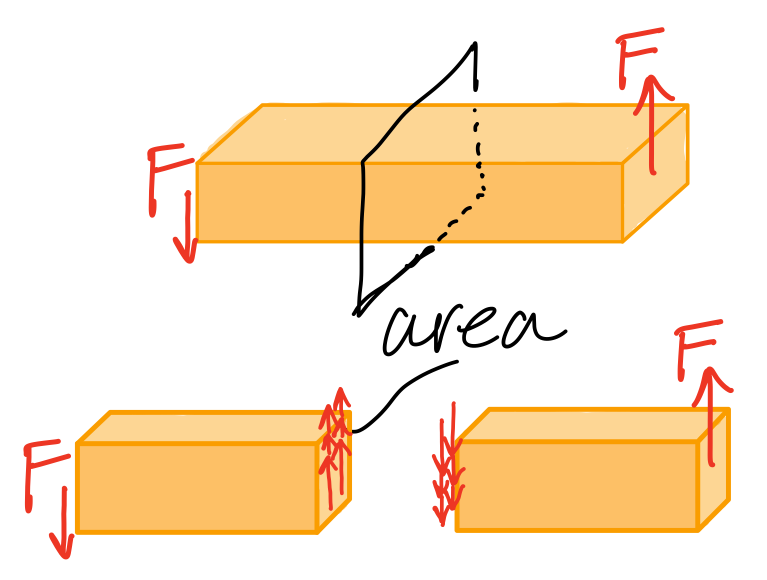
\includegraphics[angle=0, width=2in]{Stress-Figures/Shear Stress.png}
\vspace{-2mm}
\caption{\small Shear stress}
\vspace{-3mm}
\label{Fig:ShearStress}
\end{figure*}

\noindent Obtained when transverse forces are applied to a member. The distribution of shear stresses cannot be assumed uniform. Common in bolts, pins and rivets used to connect various structural members.

\begin{figure*}[!h]
\centering
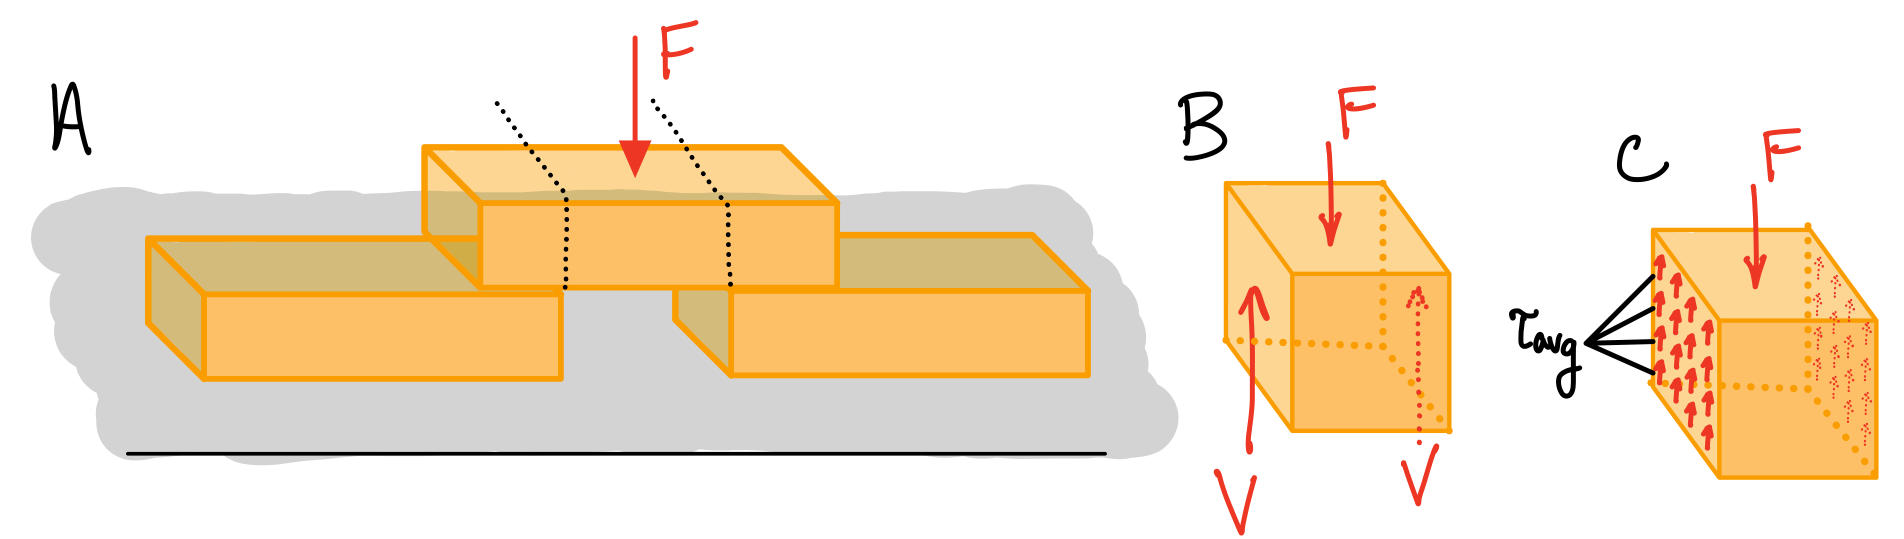
\includegraphics[angle=0, width=4in]{Stress-Figures/Avg Shear Stress.png}
\vspace{-2mm}
\caption{\small Average shear stress}
\vspace{-3mm}
\label{Fig:AvgShearStress}
\end{figure*}

\[\tau_{ave} = \frac{V}{A}\]

\noindent where $V$ is the internal resultant shear force and $A$ is the cross-sectional area of the bar where the shear stress $\tau_{ave}$ is calculated.


\vspace{5pt}

\noindent \textbf{Example:} Single Shear
Determine the shear stress in the bolt.
\begin{figure*}[!h]
\centering
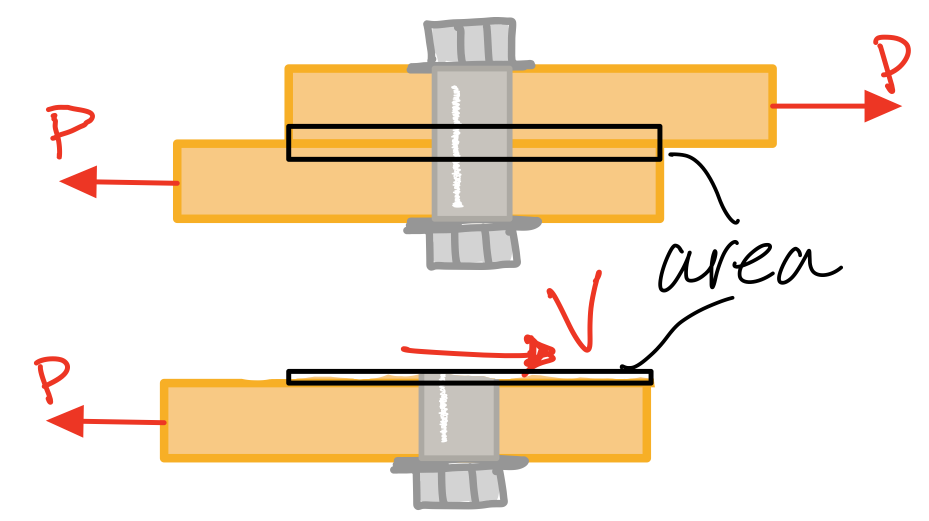
\includegraphics[angle=0, width=2.5in]{Stress-Figures/SingleShear.png}
\vspace{-2mm}
\caption{\small Single shear stress}
\vspace{-3mm}
\label{Fig:SingleShearStress}
\end{figure*}

\[\tau_{ave} = \frac{P}{A}\]
\noindent \textbf{*Expandable derivation*}
\[\Sigma F_y = V-P = 0\]
\[V = P\]

\noindent \textbf{**End Derivation**}

\noindent \textbf{Example:} Double Shear

Determine the shear stress in the bolt.
\begin{figure*}[!h]
\centering
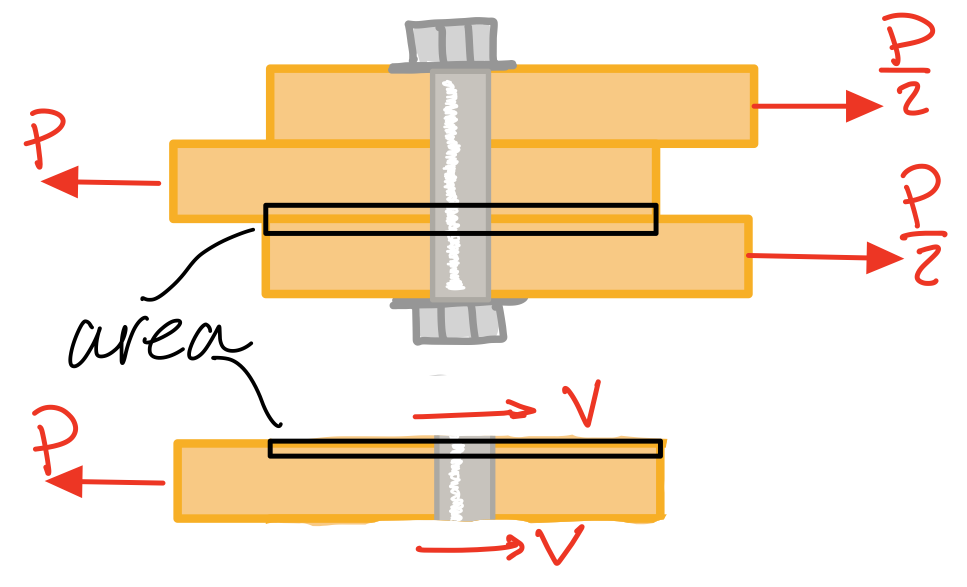
\includegraphics[angle=0, width=2.5in]{Stress-Figures/DoubleShear.png}
\vspace{-2mm}
\caption{\small Double shear stress}
\vspace{-3mm}
\label{Fig:DoubleShearStress}
\end{figure*}

\[\tau_{ave} = \frac{P}{2A}\]

\textbf{*Expandable derivation*}
\[\Sigma F_y = 2V-P = 0\]
\[V = \frac{P}{2}\]

\noindent \textbf{**End Derivation**}

\subsubsection{Stress Tensor}

\begin{figure*}[!h]
\centering
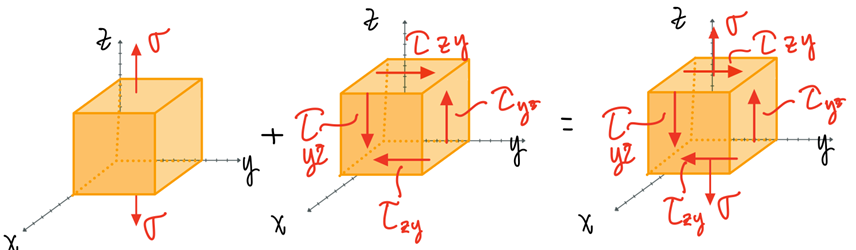
\includegraphics[angle=0, width=\columnwidth]{Stress-Figures/Stress Element.png}
\vspace{-2mm}
\caption{\small Stress element}
\vspace{-3mm}
\label{Fig:Element}
\end{figure*}

\noindent The components of normal and shear stress can be combined into the stress tensor. This is a symmetric matrix representing the state of stress with respect to three directions.

\[ T= \begin{bmatrix} \sigma_{x} & \tau_{xy} & \tau_{xz} \\ \tau_{yx}& \sigma_{y} & \tau_{yz} \\ \tau_{zx}&\tau_{zy}&\sigma_{z} \end{bmatrix} \]

% \[ T&nbsp;= \begin{bmatrix} \sigma_{x} &amp; \tau_{xy} &amp; \tau_{xz} \\ \tau_{yx}&nbsp;&amp; \sigma_{y} &amp; \tau_{yz} \\ \tau_{zx}&nbsp;&amp; \tau_{zy}&nbsp;&amp; \sigma_{z} \end{bmatrix} \]

\begin{itemize}
    \item  Three normal stress components: $\sigma_x, \sigma_y, \sigma_z$
    \item Six shear stress components: $\tau_{xy} =\tau_{yx}, \tau_{xz}=\tau_{zx}, \tau_{yz}=\tau_{zy}$
\end{itemize}

\noindent The first subscript describes the surface \textbf{orientation} in the normal direction. The second subscript describes the \textbf{direction} of the stress.

\clearpage

\subsection{Support Reactions}

\begin{figure*}[!h]
\centering
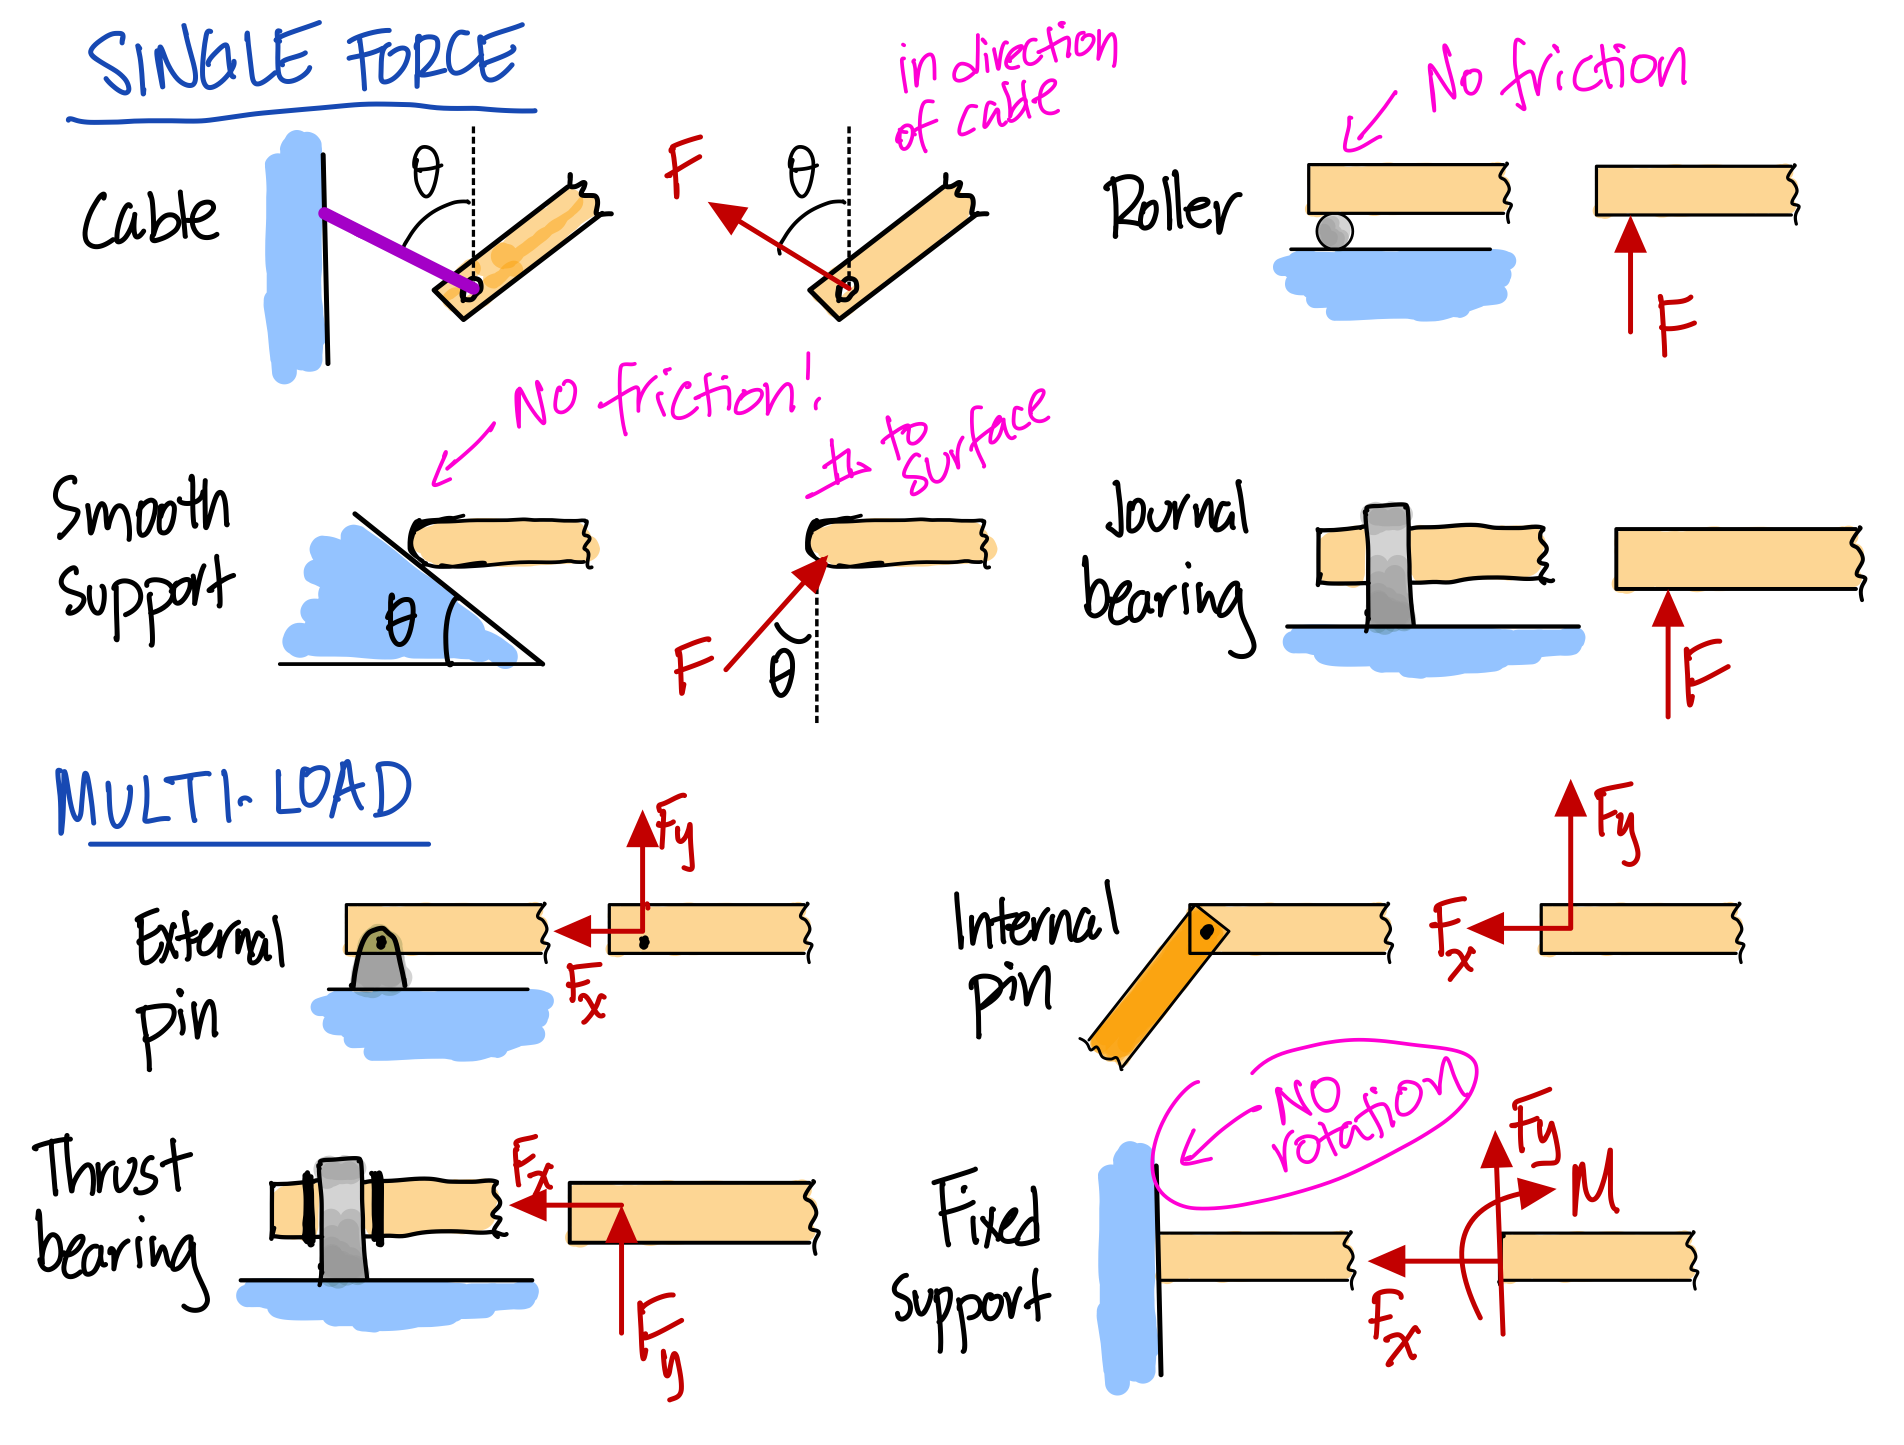
\includegraphics[angle=0, width=\columnwidth]{Stress-Figures/Support reactions.png}
\vspace{-2mm}
\caption{\small Support reactions}
\vspace{-3mm}
\label{Fig:Supports}
\end{figure*}

\subsection{Allowable Strength Design}

\textbf{Design Requirement:} A structural design is intended to support and/or transmit loads while maintaining safety and utility: \textbf{\textit{don't break}}. Strength of a structure reflects its ability to resist failure.

\begin{itemize}
    \item \textbf{Ultimate load ($P_u$):} force when specimen fails (breaks).
    \item \textbf{Ultimate normal stress ($\sigma_u$):} \[\sigma_u = \frac{P_u}{A}\]
\end{itemize}

\noindent A structure is safe if its strength exceeds the required strength.

\noindent \textbf{Factor of Safety (FS):} Ratio of structural strength to maximum (allowed) applied load ($P_{all}$).

\[P_{all} \le \frac{P_u}{FS}\]

\noindent Similarly, \[\sigma_{all} \le \frac{\sigma_u}{FS}\]


